

\documentclass{article}
\usepackage[utf8]{inputenc}
\usepackage{fullpage}
\usepackage{graphicx}
\usepackage{wrapfig}
\usepackage{caption}

\begin{document}

\pagenumbering{gobble}

\begin{center}\huge{Stage de Noël 2015}\end{center}

\vspace{1cm}

\begin{wrapfigure}{l}{0.5\textwidth}
\scalebox{0.4}{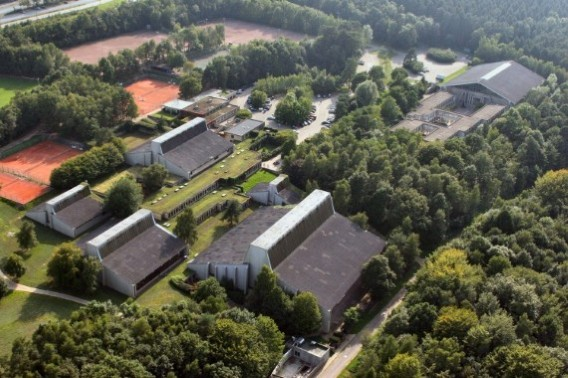
\includegraphics{adeps.jpg}}
\caption*{Centre ADEPS Le Blanc Gravier}
\vspace{-1.8cm}
\end{wrapfigure}

\paragraph{Quand?} Le stage se déroulera durant la première semaine des vacances de Noël du vendredi 18 décembre 2015, 17h au jeudi 24 décembre 2015, 14h.

\paragraph{Où?} Domaine de l'Université, Allée des Sports P63 4000 Liège, Belgique. Il s'agit du complexe sportif ADEPS Le Blanc Gravier, situé au coeur du domaine universitaire de la ville de Liège. Le centre sportif Le Blanc Gravier possède l'une des infrastructures sportives les plus complètes du pays.

\paragraph{Déplacement} Si nous manquons de place dans les voitures, un départ en transport en commun sera prévu.

\paragraph{Logements} Chambres de deux personnes.

\paragraph{Prix} Nous demandons aux parents des nageurs une participation de 140 euros par nageur. Pour information, le coût total du stage s'élève à environ 240 euros pour le logement, la nourriture et la location de la piscine (2 couloirs). {\bf Remarque:} Si le prix du stage demeure un problème, contactez-nous! Nous voulons que tout le monde puisse participer!

\paragraph{Inscriptions} Pour marquer votre participation, il vous faudra verser (soit par virement bancaire soit en liquide) un accompte de 50 euros au club (ou directement les 140 euros!). Les inscriptions sont ouvertes jusqu'au lundi 30 novembre 2015 inclu.

\paragraph{Encadrement} Laurent et Miguel seront les deux accompagnants chargés du bon déroulement du stage.

\paragraph{Entrainement} Le but de ce stage est avant tout de s'amuser! Ceci étant dit, douze séances d'entrainement de deux heures sont prévues. Cela représente une grosse charge de travail, qui demandera toute votre motivation!

\vspace{1cm}
\hspace{-0.66cm} Pour toutes informations complémentaires, veuillez contacter Laurent Christophe: \texttt{lachrist@vub.ac.be}.
\vspace{0.7cm}

En espèrant vous-y voir nombreux(ses)!

\end{document}